\documentclass{report}

\usepackage{graphicx}
\usepackage{amsmath}
\usepackage{epstopdf}
\usepackage{url}
\usepackage{verbatimbox}
\usepackage{pdfpages}

\DeclareMathOperator*{\argmin}{arg\,min}

\title{\LARGE \bf
A Multiple-Camera System Calibration Toolbox
}

\author{
Bo Li \\ Advised by Kevin K\"oser and Marc Pollefeys\\
Computer Vision and Geometry Group\\ ETH Zurich
}

\begin{document}

\maketitle
\tableofcontents

\begin{abstract}
This thesis presents some recent developments on camera calibration. It includes the following contents: 

1) An calibration approach for multiple-camera systems. We propose a novel feature descriptor-based calibration pattern. It can be used for easily calibrating both the intrinsics and extrinsics of a multiple-camera system. The calibration only requires that neighboring cameras observe parts of the calibration pattern at the same time; the observed parts may not overlap at all. No overlapping fields of view are assumed for the camera system.

2) An open source multiple-camera system calibration toolbox for Matlab. The proposed toolbox supports the calibration of a camera system which can comprise either normal pinhole cameras or catadioptric cameras. We show that the toolbox can be easily used to automatically calibrate camera systems. 

3) Some exploration of the calibration problem in scenario of camera-display pair. 


\end{abstract}



\chapter{Introduction}
Multiple-camera systems have become increasingly prevalent in robotics and computer vision research. These systems include mature products e.g. stereo camera or Ladybug camera, and also a large variety of customized camera systems. Commonly used cameras in the systems include normal pinhole cameras, fish-eye cameras and catadioptric cameras. To make such systems to work properly, both the intrinsics and extrinsics of the cameras should be well calibrated. 

\section{Related Work}
Recently, many efficient methods have been developed for intrinsic calibration of many types of cameras. These methods can be divided into two categories: calibration with a special calibration object, and self-calibration. In this paper, we focus on the former category which is usually much more accurate than self-calibration. Many toolboxes are available for this category of methods. Seminal work on calibrating a pinhole camera can be found in \cite{zhang2000flexible}. Some popular calibration toolboxes \cite{bouguet2004camera,stoyanov2006camera} are inspired by this method. For generic cameras, \cite{scaramuzza2006toolbox} proposes a toolbox to use a polynomial to approximate rays corresponding to each image point. This method generically applies to most camera models but does not provide a closed-form solution for undistorting raw images. In the toolbox proposed in \cite{mei2007single}, an unified projection model is proposed for calibrating a catadioptric system, fish-eye camera and sphere mirror system. This model is similar with \cite{scaramuzza2006toolbox} but parameterizes rays instead of using an arbitrary polynomial, which makes undistortion much simpler. Details about the previous intrinsic calibration methods can be found in section \ref{}. 

Some toolboxes are also available to calibrate simple multiple-camera systems. \cite{bouguet2004camera} enables one to calibrate a stereo camera. For calibration with a system of more than two cameras, these toolboxes \cite{svoboda2005convenient,easycal} can be used. These calibration toolboxes make use of the overlapping fields of view of the cameras; hence, these toolboxes can calibrate a stereo camera and a circular camera rig with all cameras pointing inwards. However, these toolboxes are not suitable for calibrating a system of cameras with no or minimal overlapping fields of view. There is increasing popularity of the use of a camera rig with cameras pointing outwards in both academia and industry; this system cannot be easily calibrated using existing calibration toolboxes due to the minimal overlapping fields of view. Hand-eye calibration algorithms \cite{tsai1989new,shiu1989calibration} can be used to calibrate this system but requires reconstructing visual odometry for each camera, and the calibration is often not accurate due to visual odometry drift. Details about some existing multiple-camera calibration methods can be found in section \ref{}. 

In addition to camera models, research has also focused on development of easy-to-use calibration patterns. Early research made use of cubes with either a chessboard pattern or circular dots on their surfaces \cite{bouguet2004camera}. This pattern is not very convenient since a perfect cube is not easy to build. Current state-of-art calibration systems mainly make use of calibration boards which are often planes with a chessboard or circular dots printed on them. An automatic detector for such patterns is readily available \cite{rufli2008automatic}. A comparison of calibration accuracy between a chessboard and circular dots can be found in \cite{mallon2007pattern}. \cite{easycal} uses a similar but even more simplified calibration object, a single point light, for calibrating multiple-camera system. One disadvantage of these patterns is that the entire pattern has to be visible in each calibration image; this requirement excludes cameras with minimal overlapping fields of view. In addition to the chessboard and circular dots, some other patterns have been proposed. \cite{schmalz2011camera} uses a temporal coded pattern to calibrate cameras. This method uses the Gray code to match world points and image points, thus not requiring the entire pattern to be in the image. The drawback of this method is the limited flexibility; the calibration requires both a display projector and a tripod for mounting a camera. More details about calibration pattern design can be found in section {}. 

\section{Motivation}
Existing calibration toolboxes using the chessboard and circular-dot patterns offer ease-of-use and high calibration accuracy when it comes to calibrating single and stereo cameras. However, for a system with multiple cameras pointing in different directions, it is difficult to use these toolboxes to calibrate the extrinsics of the camera system. This is because current automatic and semi-automatic chessboard detectors require the chessboard to be entirely within the field of view of the cameras. Therefore, if two cameras have minimal overlapping field of view, it is difficult to use the chessboard for extrinsic calibration in contrast to stereo camera calibration. The extrinsic calibration for cameras with minimal overlapping fields of view can be made easier if we relax the requirement that the calibration pattern be seen in its entirety by each camera; ideally, the calibration board is automatically detected even when the cameras observe different parts of the board. For most multiple-camera systems, it is fairly common for a camera pair to see different parts of a suitably-sized calibration board at the same time. Based on this motivation, we design a feature descriptor-based calibration pattern which is easy to detect even when seen partially by a camera, and a extrinsic calibration framework using this pattern. 



\section{Contributions}

The main part of this thesis makes two novel contributions: 

\begin{enumerate}
\item A new calibration pattern that encodes feature points using feature extraction techniques. Our pattern contains a large number of detectable features on multiple scales, as illustrated in chapter \ref{PatternSec}. The pattern can be recognized and localized even if the pattern is partially seen in an image. 
\item A toolbox based on the proposed calibration pattern. This toolbox can be used for both intrinsic and extrinsic calibration of a multiple-camera system, as illustrated in chapters \ref{singleSec} and \ref{extrinsicSec}. Similarly to existing calibration toolboxes, our toolbox can also be used for intrinsic calibration of a single camera. 
\end{enumerate}

 

\chapter{Calibration Pattern}
\section{Introduction}
%TODO 1. 3D chessboard; 2. chessboard and dot; 3. Temporal code and bar code; 4. Random dots; 5. Pattern using rank. 
The basic usage of a calibration pattern is to provide easy-to-detect feature points with known 3D coordinates. These features are then detected in the images taken by the camera to be calibrated. The corresponding 2D and 3D points can then be used to estimate the camera parameters. 

Early calibration research, for example the ?DLT? method (see section \ref{} for more details), uses a cube with gridded squares or dots printed on it as the calibration pattern object \cite{}. Three orthogonal edges of the cube defines the three axes of a world coordinate system. Coordinates of the square corners or the dots can be easily measured. Figure \ref{} shows an example of the calibration cube. The usage of the calibration cube is limited by two drawbacks: 1) It is not flexible and convenient to build and move a large cube; 2) It is difficult to build a cube with its edges perfectly orthogonal. 

As later research proposes efficient calibration method using 3D points from only one plane, plane calibration objects become most widely used in recent research on camera calibration. A variety of 2D calibration patterns are proposed. Here we provide an overview of some existing 2D calibration pattern. This overview compares the patterns in the following two aspects: 1) The accuracy of feature detection; 2) The difficulty of automatic feature detection and matching. 

\begin{itemize}
	\item \textit{Chessboard and gridded dots} Figures \ref{} and \ref{} show images of the two patterns. These pattern the most widely used calibration pattern in current camera calibration research. Discussion about the accuracy of these two pattern can be found from \cite{mallon2007pattern}. The chessboard corner detection is well-known to be very sub-pixel accurate and unbiased, while the dot detection maybe biased due to the distortion of the cameras. Automatic detection for this two pattern is both possible and many available detection package can be obtained online. %TODO All the matlab chessboard detection links and dot detection links. 
	
\end{itemize}

\begin{figure}
\centering
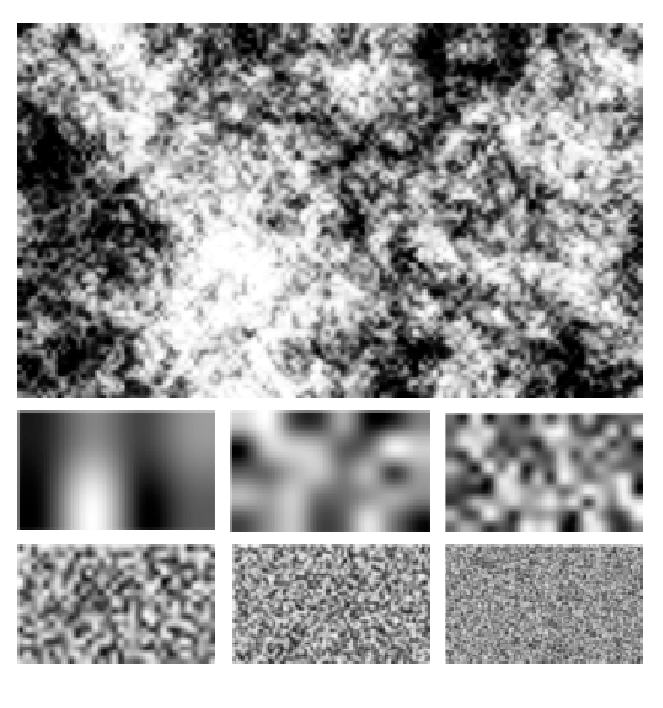
\includegraphics[width=0.6\textwidth]{images/patternsample}
\caption{Top: The proposed calibration pattern. Bottom: Image components with noise at different frequencies.}
\label{PatternFig}
\end{figure}


\label{PatternSec}
\section{Feature Detection Revisited}
%TODO Added sift feature figures and more details. 

Point-feature detection is a computer vision technique widely and successfully applied to many areas such as sparse reconstruction and object detection. A point feature typically contains two components: a keypoint and a descriptor. We look at the widely-used SIFT implementation \cite{lowe2004distinctive} as a example. A Difference of Gaussian filter (DoG) is used to detect key points. This detection is executed on both the original image and downsampled images; in short, keypoint detection is done on different scales. For each keypoint, the image gradient in the keypoint's neighborhood is converted to a histogram which is then used as the descriptor for the corresponding feature point. SURF, a variant of SIFT, is also a widely-used feature detection and descriptor extraction technique \cite{bay2006surf}. SURF replaces SIFT in many applications due to the its computational efficiency. In the proposed toolbox, we use SURF features. 

\section{Reverse Engineering}
The basic idea behind the proposed calibration pattern is to find and design a pattern that yields a high number of detectable features. At the same time, the feature descriptors should be highly discriminative so that we can easily obtain unique feature point matches. 

To facilitate feature detection, we use several noise images to compose a calibration pattern in accordance with the mechanism of SIFT/SURF. The DoG filter applied to a noise image can yield points with high response. However, a problem with high-frequency image noise is the blurring effect. For a grayscale image, if the camera is located far away, the noise image is perceived as a purely gray image. The solution to this problem is to compose images with noise from multiple scales. In our implementation, we generate noise images of different sizes, and resize them such that they have the same size. These images with noise on different scales are then added up together. This procedure can be interpreted as a reverse engineering of the scaling procedure in SIFT/SURF detection. Thus, the resulting image contains a high number of detectable features on different scales; such features can be detected by a camera at varying distances. The following Matlab code generates a $600 \times 800$ calibration pattern. Figure \ref{PatternFig} shows a calibration pattern at the top, and its components with noise on different scales at the bottom. 

\small
\begin{verbbox}
N = 600; M = 800;
pattern = 0; count = 0;
m = 4;
while m < M
  n = round(N / M * m);
  noise = rand(n, m);
  noise = imresize(noise, [N, M]);
  pattern = pattern + noise;
  count = count + 1;
  m = m * 2;
end
pattern = pattern ./ count;
pattern = histeq(pattern);
imshow(pattern);
\end{verbbox}
\normalsize

\begin{figure}
  \centering
  \theverbbox
  \caption{Matlab code for pattern generation.}
\end{figure}


\section{Feature Matching}
Feature detection and feature matching between two images are two standard steps of in a modern 3D vision pipeline. In our calibration approach, we employ a similar step to match features between each image and the known calibration pattern image. First, features detected from each image and the pattern image are matched according to the descriptor similarity. We use the well-known distance ratio check proposed in \cite{lowe2004distinctive}. For a set of at least 2 candidate matches for each query feature, the best match is accepted only if its descriptor distance is smaller than 0.6 times the descriptor distance between the query feature and its second best match. 

Next, a \textit{fundamental matrix for radial distortion} is estimated by RANSAC between the image points and pattern points to find inlier point correspondences. Note that this fundamental matrix is not the same matrix used in traditional epipolar geometry. The traditional matrix requires that point correspondences have image coordinates corresponding to rectified images. Details about this fundamental matrix can be found in \cite{hartley2007parameter}. We provide some simple explanation about the fundamental matrix here. Denote $p^d$ as a distorted image point, $p^u$ as its corresponding undistorted point and $p^c$ as the corresponding point on the calibration pattern. If the image only has radial distortion and $e$ is the distortion center, we can write:
\begin{equation}
p^d = e + \lambda (p^u - e)
\end{equation}
where $\lambda$ is a distortion coefficient corresponding to $p^u$. In addition, since $p^u$ can be obtained by a perspective transform from $p^c$, there exists a homography $H$ such that $p^u = H p^c$. Substituting this into the above equation, we obtain: 
\begin{equation}
p^d = e + \lambda (H p^c - e)
\end{equation}
Left-multiplying the equation by $[e]_\times$, we get:
\begin{equation}
{}[e]_\times p^d = \lambda [e]_\times H p^c
\end{equation}
Left-multiplying the equation again by ${p^d}^\top$, we get:
\begin{equation}
0 = {p^d}^\top [e]_\times H p^c
\end{equation}
$F \equiv [e]_\times H$ is the fundamental matrix for radial distortion, and $e$ can be interpreted as the principal point. This fundamental matrix is well-suited to both the pinhole and unified projection models, and is used to remove false feature matches in our proposed calibration approach. Only in case the images perfectly agree with the pinhole camera model (no lens distortion at all), it suffices to estimate a homography.
This case could be detected by automatic model selection methods like the GRIC criterion\cite{torr1997assessment}, however since this is a very special case, for the current version we leave it to the user to specify this mode.
% However, this fundamental matrix for radial distortion is degenerate when the features are perfectly undistorted. In this case, a homography can be estimated between the pattern features and image features. We select the correct model by comparing the number of inliers.  investigates more complex model selection methods; however, we do not use such methods in our toolbox for sake of simplicity. 

\chapter{Single-Camera Calibration}
\section{Introduction}
%TODO 0. DLT method; 1. Zhang's model; 2. Scaramuzza and Mei. 


\label{singleSec}
A single-camera calibration estimates the camera intrinsics and the poses of the calibration pattern with respect to the camera's coordinate system. This data from the single-camera calibration is used by the multiple-camera extrinsic calibration. 
\section{Camera Model}
\subsection{Pinhole Camera Model}
We consider the mostly commonly used pinhole camera projection model first and introduces the notations. A homogeneous 3D point $(X, Y, Z, 1)$ is projected onto a homogeneous image point $(u, v, 1)^\top$ via: 
\begin{eqnarray}
\begin{bmatrix}
	\begin{array}{c}
	x \\ y \\ z
	\end{array}
\end{bmatrix} 
&=&
\begin{bmatrix}
R & t
\end{bmatrix}
\begin{bmatrix}
	\begin{array}{c}
	X \\ Y \\ Z \\ 1
	\end{array}
\end{bmatrix} \\
\label{cmEqn1}
x' &=&x / z \\ 
\label{ray2homo1}
y' &=&y / z \\
\label{ray2homo2}
x'' &=&x'  + dx_{\text{radial}} + dx_{\text{tangent}}\\
\label{cmEqn2}
y'' &=&y'  + dy_{\text{radial}} + dy_{\text{tangent}}\\
\label{cmEqn3}
\begin{bmatrix}
	\begin{array}{c}
	u \\ v \\ 1
	\end{array}
\end{bmatrix} 
&=&
K
\begin{bmatrix}
	\begin{array}{c}
	x'' \\ y'' \\ 1
	\end{array}
\end{bmatrix}
\label{cmEqn4} 
\end{eqnarray}

where $R$ and $t$ are the rotation and translation from the world frame to the camera frame. 

The lens distortion of common pinhole camera model consists of radial distortion and tangent distortion. The radial distortion is used to model the imperfection of the lens shape; the tangent distortion is used to model the assembly deviation of the lens and the camera. The radial and tangent distortion is formed as: 
\begin{eqnarray}
\begin{bmatrix}
	\begin{array}{c}
	dx_{\text{radial}} \\ dy_{\text{radial}}
	\end{array}
\end{bmatrix} 
&=&
(1 + k_1 \rho^2 + k_2 \rho^4) 
\begin{bmatrix}
	\begin{array}{c}
	x' \\ y'
	\end{array}
\end{bmatrix} \\
\begin{bmatrix}
	\begin{array}{c}
	dx_{\text{tangent}} \\ dy_{\text{tangent}}
	\end{array}
\end{bmatrix} 
&=&
\begin{bmatrix}
	\begin{array}{c}
	2 p_1 x' y' + p_2 (\rho^2 + 2 x'^2) \\ 
	p_1 (\rho^2 + 2 y'^2) + 2 p_2 x' y'
	\end{array}
\end{bmatrix} \\
\rho &=& \sqrt{x'^2 + y'^2}
\end{eqnarray}

$K$ is the intrinsic matrix denoted as: 
\begin{equation}
K = 
\begin{bmatrix}
	\begin{array}{ccc}
	\gamma_1 & s & u_0 \\ 
	0 & \gamma_2 & v_0 \\ 	
	0 & 0 & 1
	\end{array}
\end{bmatrix}
\end{equation}
where $\gamma_1$ and $\gamma_2$ are the focal lengths of horizontal and vertical directions; $s$ is the skew parameter; $(u_0, v_0)^\top$ is the principal point. 

Details about the pinhole camera model can be found from \cite{hartley2000multiple}. Details about the distortion model can be found from \cite{}. 

\subsection{Extension for Generic Cameras}
We can easily extend the above pinhole camera model to generic cameras. Firstly consider a ideal camera with focal length $\gamma$, principal point $(0, 0)^\top$, and without distortion. An image point $(u, v, 1)^\top$ corresponds to a ray with direction $(u, v, f(u, v))^\top$ which goes through the origin of the camera's coordinate system. This ray definition unifies the various projection models via different definitions of $f(u, v)$. For the pinhole projection model, the corresponding ray is $(u, v, \gamma) \sim (x', y', 1)$. Thus we have: 
\begin{equation}
f(u, v) \equiv \gamma
\label{pinholeEqn}
\end{equation}
For the unified projection model with its lens distortion parameter $\xi = 1$,
\begin{equation}
f(u, v) = \frac{\gamma}{2} - \frac{1}{2 \gamma} \rho^2
\label{parabolaEqn}
\end{equation}
where $\rho = \sqrt{u^2 + v^2}$. Details about equation \ref{parabolaEqn} can be found in \cite{mei2007single}. For the Taylor projection model, $f(u, v)$ is parameterized as a general polynomial with one variable $\rho$, as proposed in \cite{scaramuzza2006toolbox}: 
\begin{equation}
f(u, v) = a_0 + \cdots + a_n \rho^n
\label{polynEqn}
\end{equation}
Equation \ref{polynEqn} does not have a closed-form inverse transform. In the proposed toolbox, we use the unified projection model in \cite{mei2007single} to model a varying range of cameras which include but are not limited to normal, wide-angle, fish-eye and catadioptric types. This model uses the same intrinsic parameters that the pinhole projection model uses: the focal length $(\gamma_1, \gamma_2)$, aspect ratio $s$, principal point $(u_0, v_0)$, and radial and tangent lens distortion parameters $(k_1, k_2, p_1, p_2)$. The model uses one additional parameter $\xi$ to model the omnidirectional camera effect. 

\section{Initialization}
The unified projection model of \cite{mei2007single} assumes the catadioptric coefficient $\xi = 1$ for initialization, and then, refines the estimated intrinsics and extrinsics. The initialization is very simple and can generate a good initial guess for all parameters. The limitation of the initialization is that it requires a known projection of a straight line on the pattern. Such a projection is easy to obtain for a chessboard but difficult for our proposed pattern. Fortunately, the initialization can be solved by substituting the unified projection model into the initialization of the Taylor projection model of \cite{scaramuzza2006toolbox}.

In the initialization, we assume the two focal lengths $(\gamma_1, \gamma_2)$ to be the same, the principal point to have the same coordinates as the image center, and zero lens distortion. For each detected feature point, we compute the corresponding $u$ and $v$ by subtracting the image center coordinates from the feature point's coordinates.

For a feature point with homogeneous image coordinates $p^c = [X, Y, 1]^\top$, denote its corresponding 3D point as $[X, Y, 0, 1]^\top$. The projection equation relating this 3D point to its corresponding camera ray $[u, v, f(u, v)]^\top$ is: 
\begin{align}
\arraycolsep=1.5pt%
\mu \begin{bmatrix}
	\begin{array}{c}
	u \\ v \\ f(u, v)
	\end{array}
\end{bmatrix}
&=
\arraycolsep=1.5pt%
\begin{bmatrix}
	r_1 && r_2 && r_3 && t
\end{bmatrix}
\begin{bmatrix}
	X \\ Y \\ 0 \\ 1
\end{bmatrix}\\
&= \begin{bmatrix}
	r_1 & r_2 & t
	\end{bmatrix} p^c
\end{align}
Left-multiplying the equation by $[u, v, f(u, v)]^\top_\times$, we have: 
\begin{equation}
\arraycolsep=1.5pt%
0 = [u, v, f(u, v)]^\top_\times
\begin{bmatrix}
	r_1 && r_2 && t
\end{bmatrix} p^c
\label{initEqn}
\end{equation}
Denote the rotation $r_i = [r_{1i}, r_{2i}, r_{3i}]^\top$ and the translation $t = [t_1, t_2, t_3]^\top$. The third row of equation \ref{initEqn} is independent of $f(u, v)$ and is a linear equation with respect to the unknowns $r_{11}, r_{21}, r_{12}, r_{22}, t_1, t_2$:
\begin{equation}
u (r_{21} X + r_{22} Y + t_2) - v (r_{11} X + r_{12} Y + t_1) = 0
\end{equation}
For each image pair, we can substitute the feature point correspondences into this equation and stack them as a linear system. Solving this system, we obtain $r_{11}, r_{21}, r_{12}, r_{22}, t_1, t_2$ up to a unknown scale. $r_{31}, r_{32}$ and the scale can be determined by exploiting the unit and perpendicularity constraints of $r_1$ and $r_2$. Note that multiple solutions exist at this stage; we reject the incorrect solutions after estimating the remaining unknowns $\gamma$ and $t_3$. 

Solving $\gamma$ and $t_3$ requires using the first and second row in equation \ref{initEqn}:
\begin{eqnarray}
v (r_{31} X + r_{32} Y + t_3) - f(u, v) (r_{21} X + r_{22} Y + t_2) = 0 \\ 
f(u, v) (r_{11} X + r_{12} Y + t_1) - u (r_{31} X + r_{32} Y + t_3) = 0
\end{eqnarray}

For the pinhole projection model, $f(u, v)$ is replaced by $\gamma$. Substituting $r_{11}, r_{21}, r_{12}, r_{22}, t_1, t_2$, we obtain linear equations with respect to $\gamma$ and $t_3$. The two unknowns are then solved by forming a linear system using detected multiple correspondences. 

For the unified projection model, equation \ref{parabolaEqn} is substituted into $f(u, v)$. We regard $\gamma$, $\frac{1}{\gamma}$ and $t_3$ as three unknowns and solve them by forming a linear system similar to the above. Since we ignore a constraint by treating $\gamma$ and $\frac{1}{\gamma}$ as two unknowns, the estimates are less accurate. This is not an issue for the initialization since the estimate is further refined. 

The initialization returns multiple solutions for the intrinsics and extrinsics; the correct solution can be selected by checking the reprojection error. 

The toolbox initializes $\gamma$ and the extrinsics for each input image, and selects the median of all values for $\gamma$ as the initial estimate for $\gamma$. 

\section{Refinement}
Based on the initial estimate, the toolbox then refines all intrinsics and extrinsics parameters using the Levenberg-Marquardt algorithm to minimize the sum of all reprojection errors. Further details about the optimization can be found in \cite{mei2007single} and \cite{scaramuzza2006toolbox}.




\chapter{Extrinsic Calibration}
%TODO Maybe talk about BA?


\begin{figure}
\centering
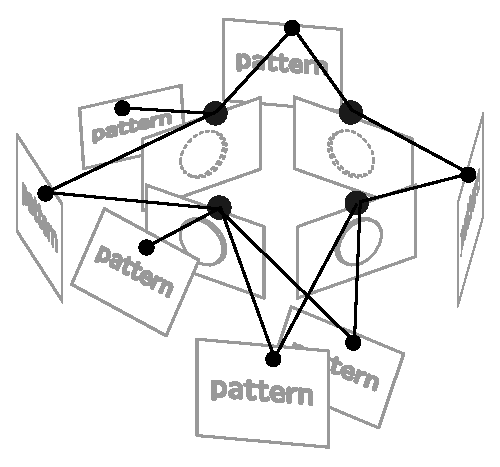
\includegraphics[width=0.6\textwidth]{images/graphsample}
\caption{A example of a pose graph for the calibration scenario of four cameras. Big dots denote camera vertices and small dots denote feature point vertices.}
\label{graphSampleFig}
\end{figure}

\label{extrinsicSec}
In this section, we assume that the cameras are rigidly mounted to a rigid body. During the image capture process, we move the calibration pattern around the camera system. The single-camera calibration provides an estimate for the poses of the calibration pattern. If the cameras are synchronized in order to take images of the pattern at the same time, the relative poses of the pattern with respect to each camera are known. Thus, the initial camera poses can be extracted from these relative poses. The toolbox optimizes the initial camera poses using a bundle-adjustment-like method. 

\section{Initialization}
We create a pose graph to denote the calibration scenario. Each camera is denoted by a camera vertex $cam_i$ in the graph. Meanwhile, each pose of the pattern is also denoted by a pattern vertex $pat_i$. If $cam_i$ takes a photo of the pattern at pose $pat_j$, then $cam_i$ and $pat_j$ are connected by an image edge denoted by $img_{i, j}$. Each edge uniquely maps to one image. Note that this graph is a bipartite graph and each edge links one camera vertex and one pattern vertex. Figure \ref{graphSampleFig} provides a simple illustration of such a graph. 

Vertices in the pose graph can be used to store the poses of the cameras and the pattern in a global coordinate system. Edges can be used to store the relative pose transform between the camera pose vertex and pattern pose vertex. For each image of the pattern at pose $pat_j$ taken by $cam_i$, we have the relative pose of $pat_j$ with respect to $cam_i$ computed from the single-camera calibration.  

Assuming that the global coordinate system is aligned with $cam_1$, the poses of all vertices connected to $cam_1$ can be obtained by following the image edges from $cam_1$. In practice, if two cameras see the pattern at the same time in their images, then the two cameras are connected via two image edges to one pattern vertex. 

Our toolbox implementation first builds a pose graph based on the results of single-camera calibration performed for all cameras. Next, a spanning tree with $cam_1$ as its root is extracted using breadth-first search. Vertex poses are then computed by traversing the spanning tree from $cam_1$ and following the image edges. In the end, we have initial pose estimates for all vertices in the global coordinate system.

\section{Refinement}
Denote the pose in the global frame of vertex $i$ (either a camera vertex or a pattern vertex) in the graph as $H_i$. On an edge $img_{i, j}$ connecting $cam_i$ and $pat_j$, the relative transform from $pat_j$ to $cam_i$ can be denoted as $H_{i, j} = H_i^{-1} H_j$. For a calibration pattern point $p^c$, its reprojection error in each image that the point is seen in is: 
\begin{equation}
e_{\textrm{reproj}}(p^c, H_{i, j}, \mathcal{I}_i) = \|\pi(p^c, H_{i, j}, \mathcal{C}_i) - p^d\|^2
\end{equation}
where $\pi$ is the image projection function corresponding to either the pinhole or unified projection model and $\mathcal{C}_i$ denotes the intrinsics of $cam_i$. $p^d$ is the distorted image point corresponding with $p^c$. 

The initial calibration estimate is refined to minimize the summation of all reprojection errors. The refinement can be over either all vertex poses or over both vertex poses and intrinsics. The optimization problem with only vertex poses is defined as: 
\begin{equation}
\begin{aligned}
& \argmin_{H_i, i > 1} & & \sum_{img_{i, j}} \sum_{k} e_{\textrm{reproj}}(p^c_k, H_i^{-1} H_j, \mathcal{C}_i) 
\end{aligned}
\end{equation}
while the optimization problem with both vertex poses and intrinsics is: 
\begin{equation}
\begin{aligned}
& \argmin_{H_i, \mathcal{C}_1, \mathcal{C}_i, i > 1} & & \sum_{img_{i, j}} \sum_{k} e_{\textrm{reproj}}(p^c_k, H_i^{-1} H_j, \mathcal{C}_i) 
\end{aligned}
\end{equation}
The optimization is over $H_i$ with $i > 1$, since $H_1 \equiv I_{4 \times 4}$ is the reference frame. The toolbox executes the optimization using the Levenberg-Marquardt algorithm. 


\chapter{Experiments}
We carry out two experiments with our proposed calibration pattern and toolbox. In the first experiment, we use a stereo camera and compare the calibration results from our toolbox and those from the OpenCV-based chessboard calibration. In the second experiment, we use our toolbox to calibrate a four-camera system. The latter camera system is a challenging case, especially for existing multiple-camera calibration methods. 

\begin{figure}
\centering
%\begin{tabular}{cc}
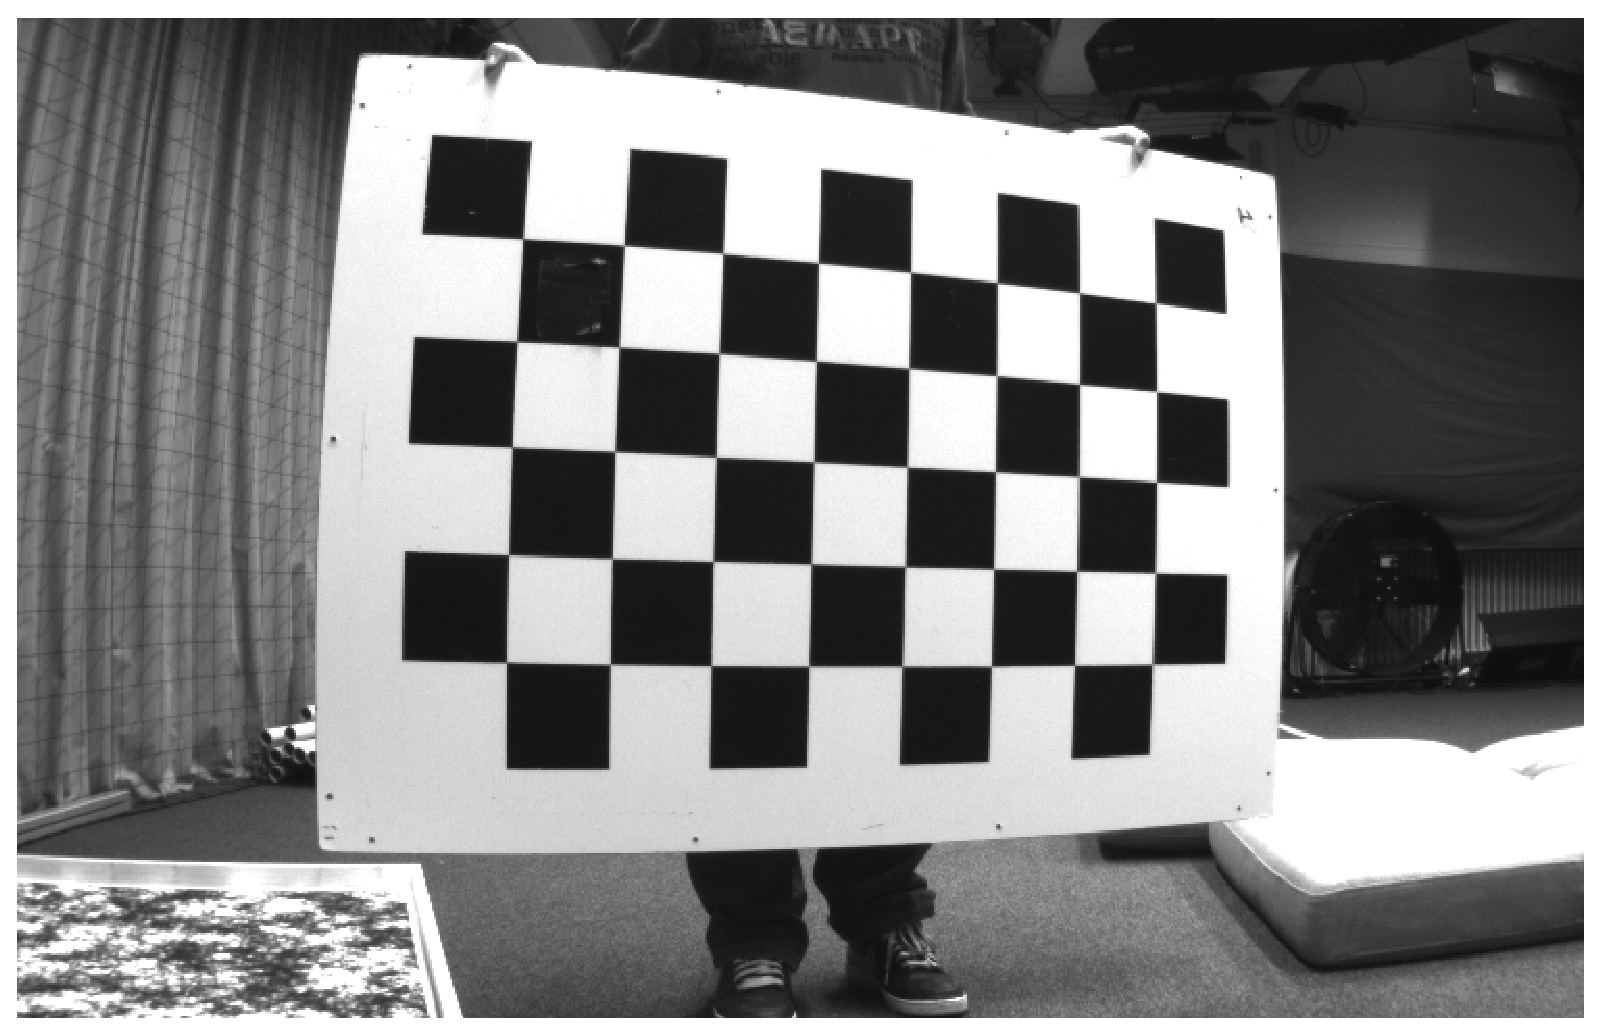
\includegraphics[width=0.4\textwidth]{images/left000} 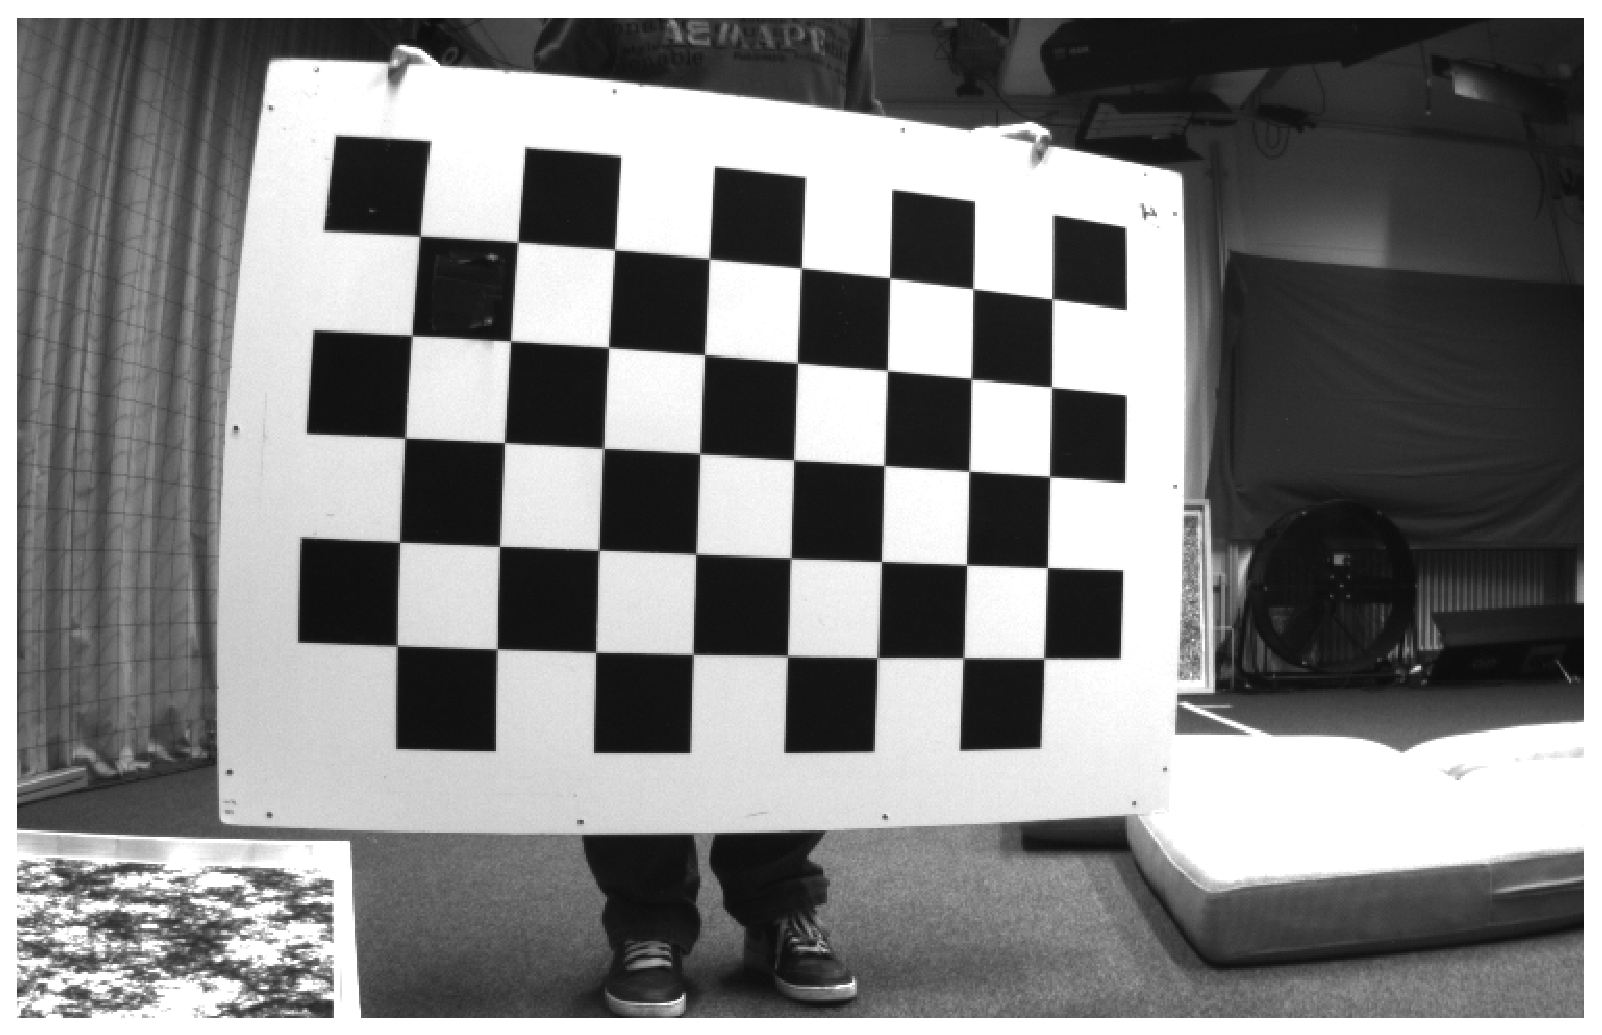
\includegraphics[width=0.4\textwidth]{images/right000} \\ 
\vspace{3pt}
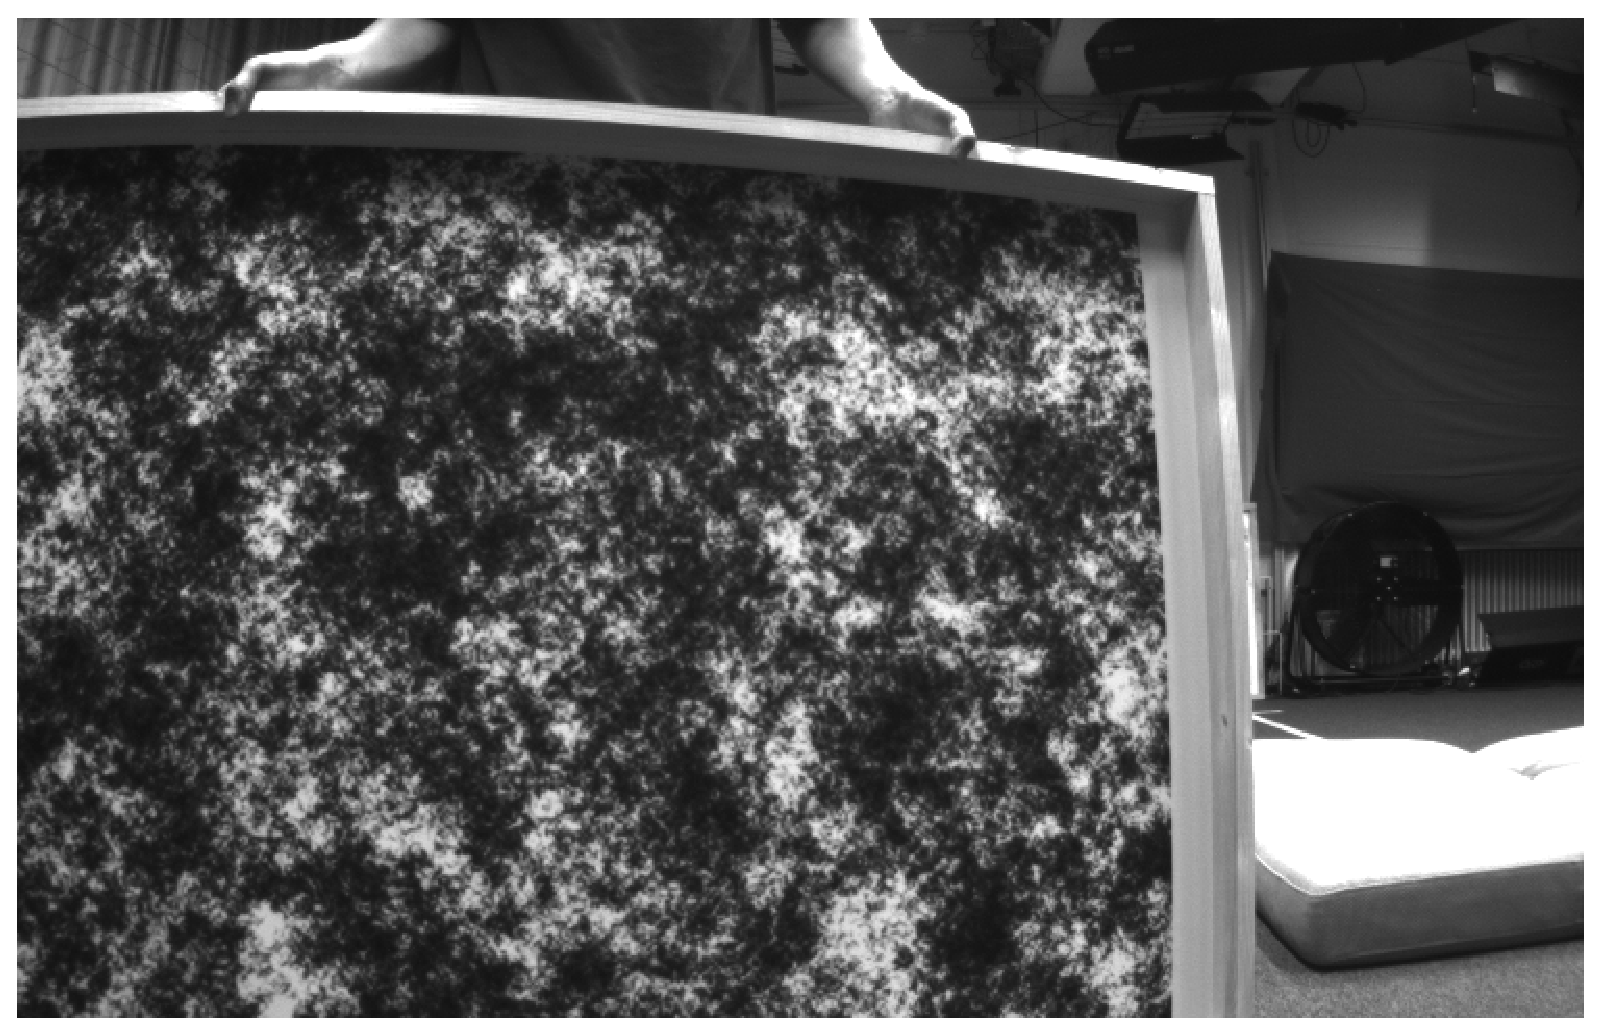
\includegraphics[width=0.4\textwidth]{images/left001} 
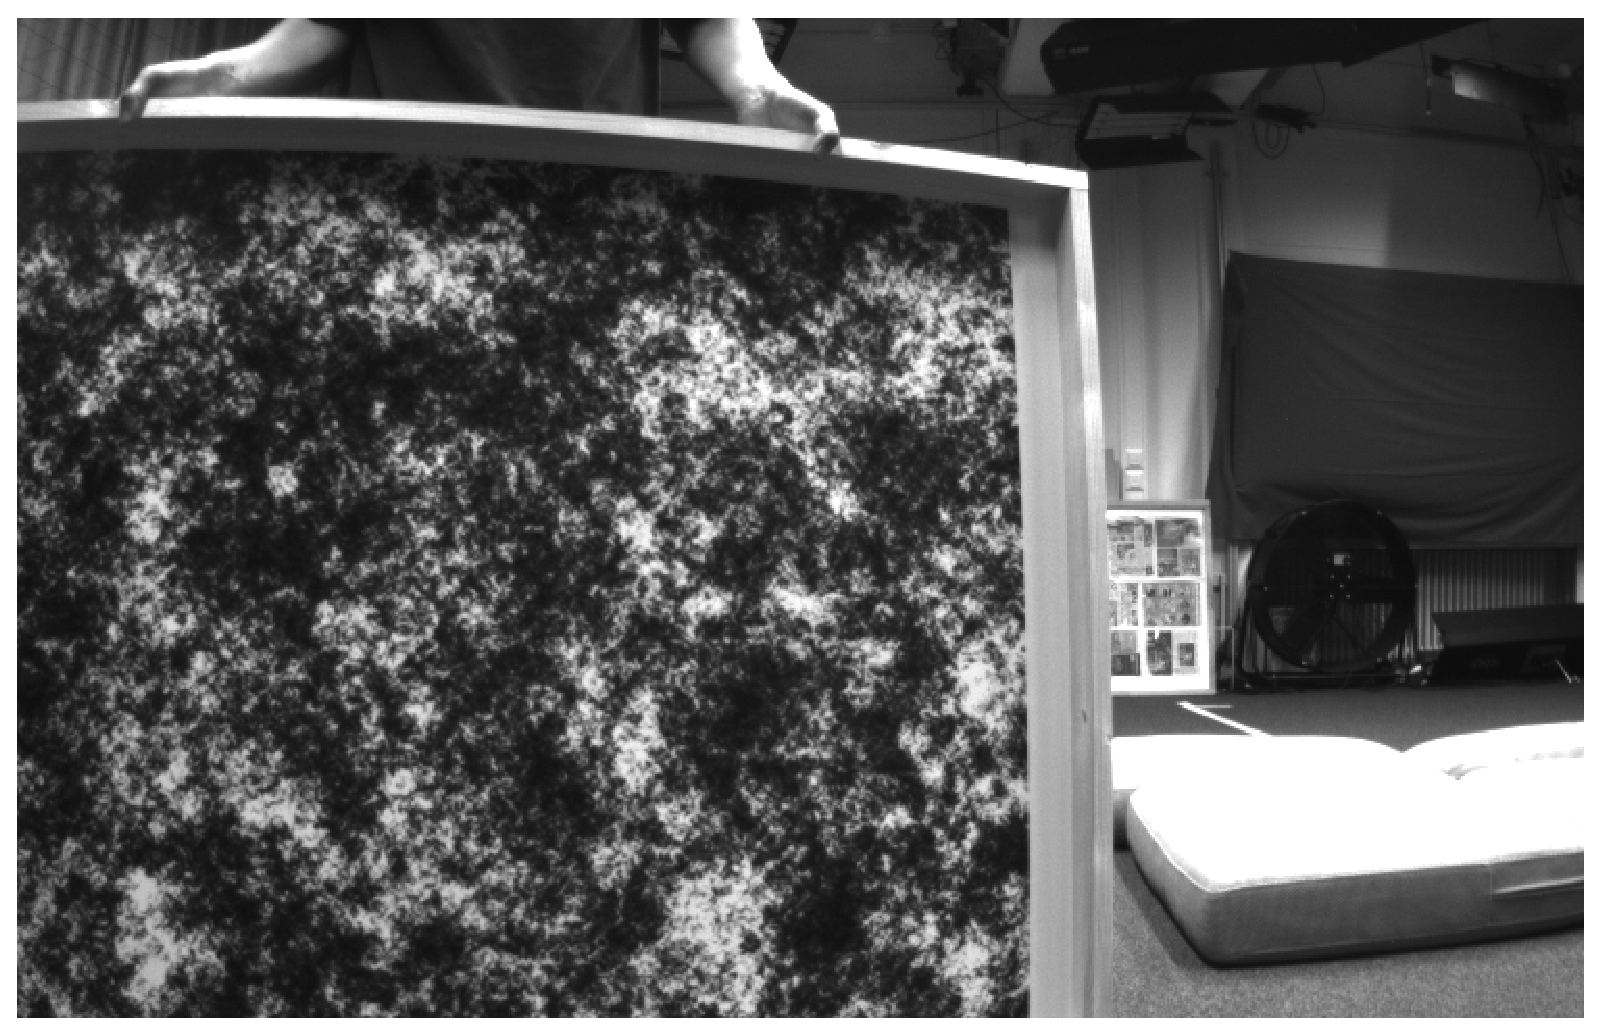
\includegraphics[width=0.4\textwidth]{images/right001} 
%\end{tabular}
\caption{Sample images used to calibrate the stereo camera. The top row shows a chessboard used by the chessboard calibration while the bottom row shows our calibration pattern used by our calibration toolbox. }
\label{stereoImageFig}
\end{figure}



\begin{figure}
\centering
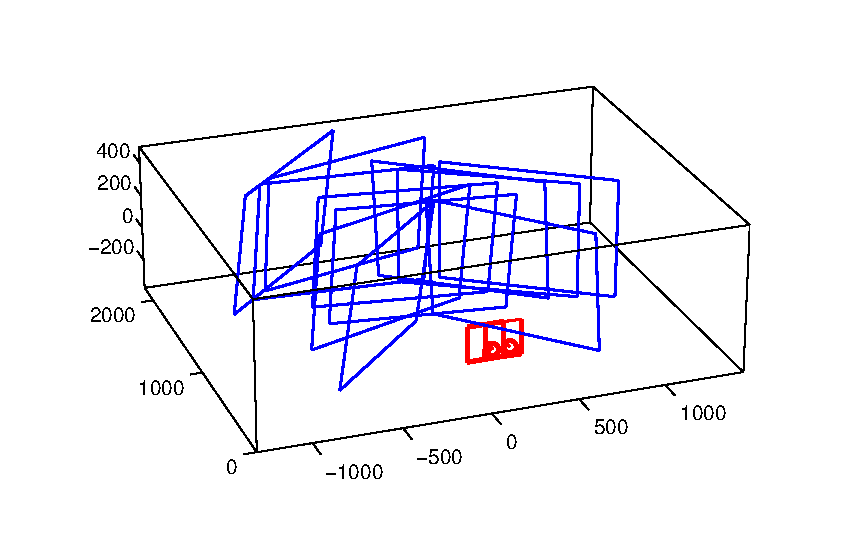
\includegraphics[trim=0in 0.1in 0in 0in, clip=true, width = 0.8\textwidth]{images/stereo3dbold}
\caption{3D plot of stereo camera and calibration pattern poses generated by our toolbox.}
\label{stereoPlot}
\end{figure}

\begin{table}
\centering
\begin{tabular}{|c|c|c|}
\hline
Object & Descriptor-based pattern & $5 \times 8$ chessboard \\
\hline
\begin{tabular}{c}
Image 
size
\end{tabular} & $480 \times 752$ & $480 \times 752$ \\
\hline
{\#} images & $10 \times 2$ & $30 \times 2$\\
\hline
\begin{tabular}{c}
{\#} features \\
(L/R)
\end{tabular} & 3073 / 2942 & 1200 / 1200 \\
\hline
\begin{tabular}{c}
Focal \\
length (L)
\end{tabular} & $(720, 718)$ & $(720, 722)$ \\
\hline
\begin{tabular}{c}
Focal \\
length (R)
\end{tabular} & $(709, 706)$ & $(709, 710)$ \\
\hline
\begin{tabular}{c}
Principal \\
point (L)
\end{tabular} & $(383, 249)$ & $(392, 250)$ \\
\hline
\begin{tabular}{c}
Principal \\
point (R)
\end{tabular} & $(387, 242)$ & $(389, 249)$ \\
\hline
\begin{tabular}{c}
Rotation \\
vector
\end{tabular} & $\left[0.001, -0.010, 0.011\right]$ & $\left[0.004, -0.009, 0.011\right]$ \\
\hline
\begin{tabular}{c}
Translation\\
vector (unit)
\end{tabular} & $\left[-1.00, -0.012, 0.005\right]$ & $\left[-1.00, -0.011, 0.012\right]$ \\
\hline
\begin{tabular}{c}
Reprojection \\
error 
\end{tabular} & 0.4 px & 0.2 px \\
\hline
\end{tabular}
\caption{Comparison of results from our method and OpenCV-based chessboard calibration for a stereo camera.}
\label{comparisonTab}
\end{table}

\section{Calibration of a Stereo Camera}
For the case of a stereo camera, a chessboard is typically used for extrinsic calibration. The two cameras tend to have a large overlapping field of view, and the entire chessboard has to be in both cameras' fields of view. We test our toolbox with a custom-built stereo camera comprising two mvBlueFOX cameras with hardware synchronization. Figure \ref{stereoImageFig} shows a sample stereo image pair used for each calibration. Note that in contrast to the chessboard calibration, our proposed calibration pattern does not have to be entirely within the field of view. The calibration results are shown in table\ref{comparisonTab}. The descriptor-based pattern provides many more features with significantly fewer images compared to the chessboard pattern. We observe that the two calibration results are very similar. The reprojection error for our proposed pattern is higher than that for the chessboard; SURF feature detection is slightly less accurate than sub-pixel chessboard corner detection in terms of feature location. For features on a coarser scale, the higher corresponding error of the estimated feature coordinates may increase the overall reprojection error. We visualize the results of our toolbox calibration in figure \ref{stereoPlot}.


\begin{figure}
\centering
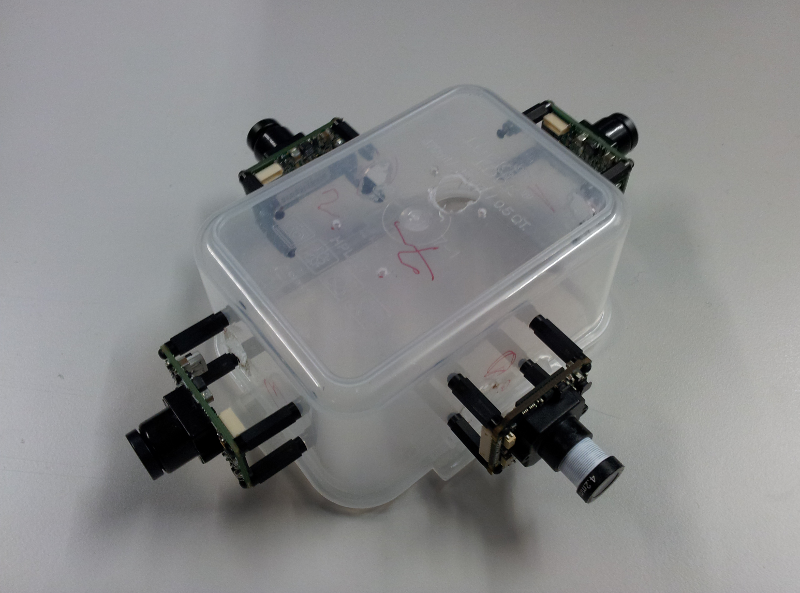
\includegraphics[width=0.7\textwidth]{images/fourcamerarig}
\caption{A four-camera system with an approximate 90\ensuremath{^\circ} relative rotation between each pair of neighboring cameras.}
\label{fourCameraRigPhoto}
\end{figure}

\begin{figure}
\centering
%\begin{tabular}{cc}
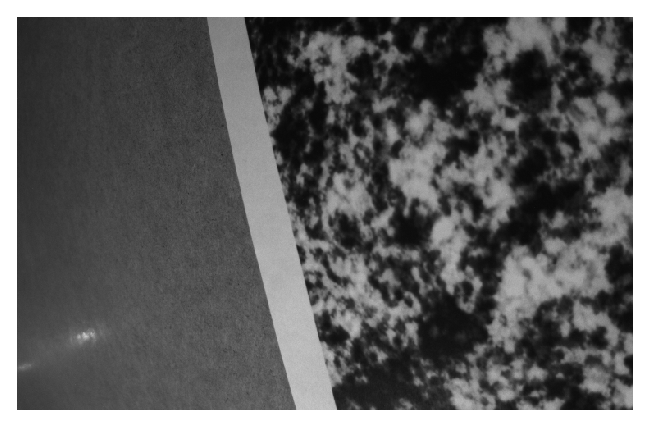
\includegraphics[width=0.23\textwidth]{images/cam4rig/1} 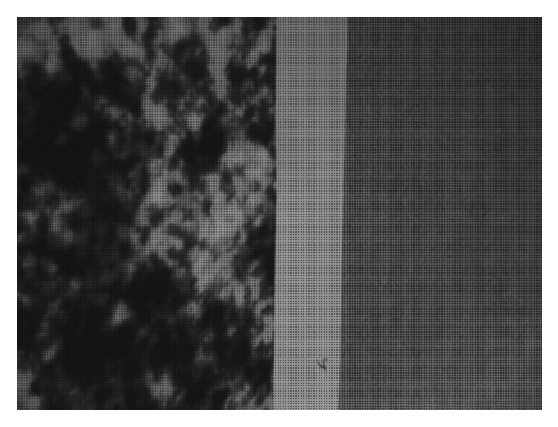
\includegraphics[width=0.23\textwidth]{images/cam4rig/2} \hspace{2pt}
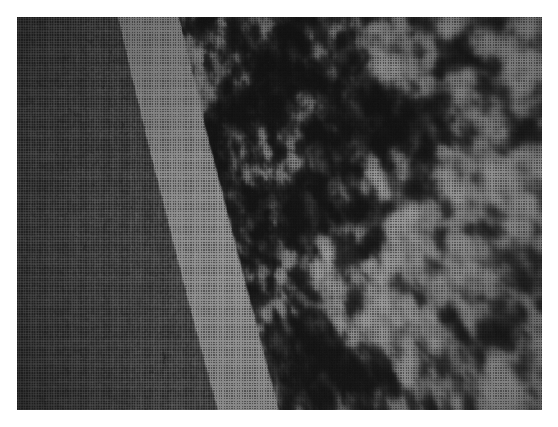
\includegraphics[width=0.23\textwidth]{images/cam4rig/3}
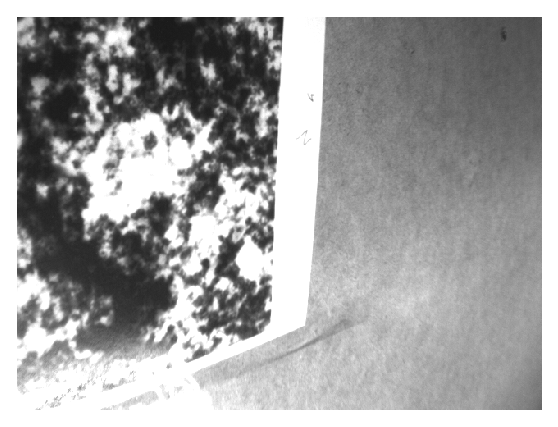
\includegraphics[width=0.23\textwidth]{images/cam4rig/4} \\
\vspace{8pt}
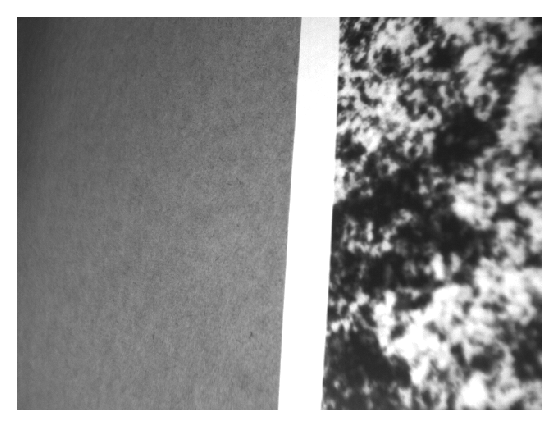
\includegraphics[width=0.23\textwidth]{images/cam4rig/5} 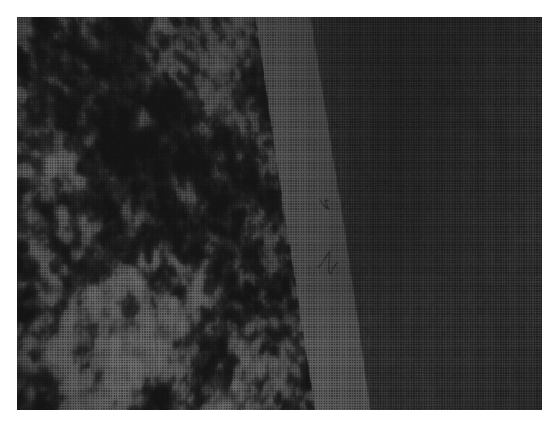
\includegraphics[width=0.23\textwidth]{images/cam4rig/6} \hspace{2pt}
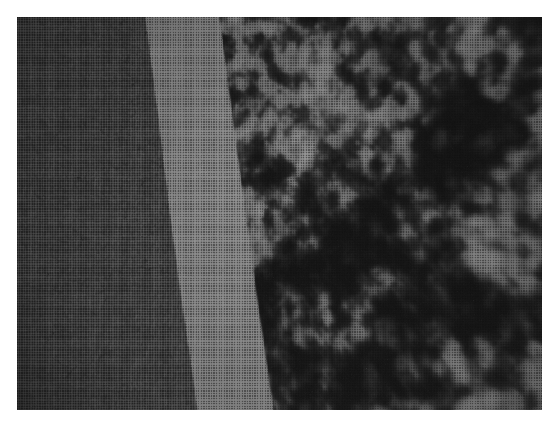
\includegraphics[width=0.23\textwidth]{images/cam4rig/7}
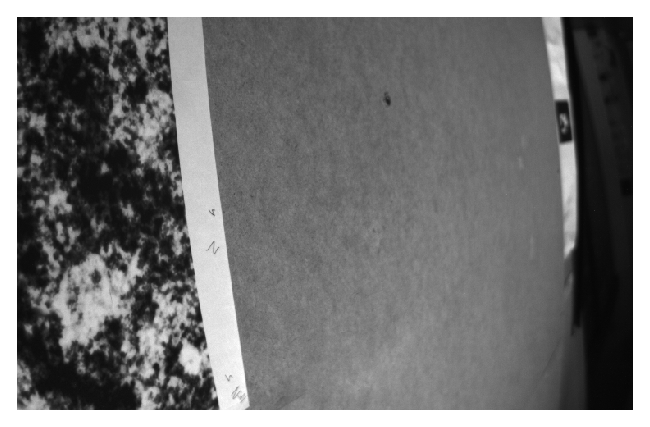
\includegraphics[width=0.23\textwidth]{images/cam4rig/8} \\%\end{tabular}
\caption{Sample images used to calibrate the four-camera rig. Each pair corresponds to an image pair from a different pair of neighboring cameras. Top-left: camera 1 and camera 2. Top-right: camera 2 and camera 3. Bottom-left: camera 3 and camera 4. Bottom-right: camera 4 and camera 1. Note that camera 1 has different resolution with the other three cameras. }
\label{fourCameraRigImageFig}
\end{figure}

\begin{figure}
\centering 
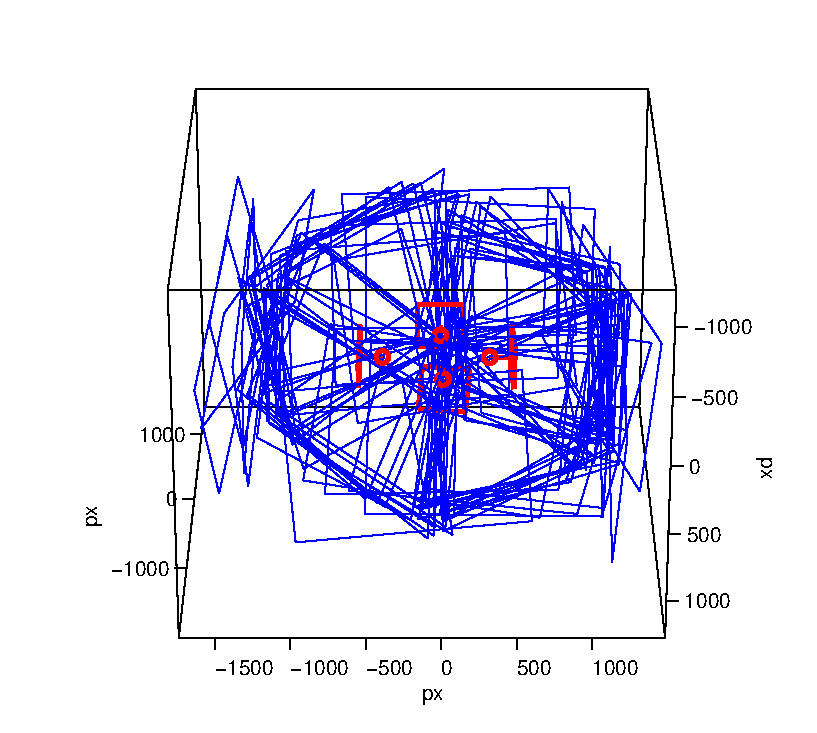
\includegraphics[trim=0in 0in 0in 0.4in, clip=true, width=0.49\textwidth]{images/rig2} 
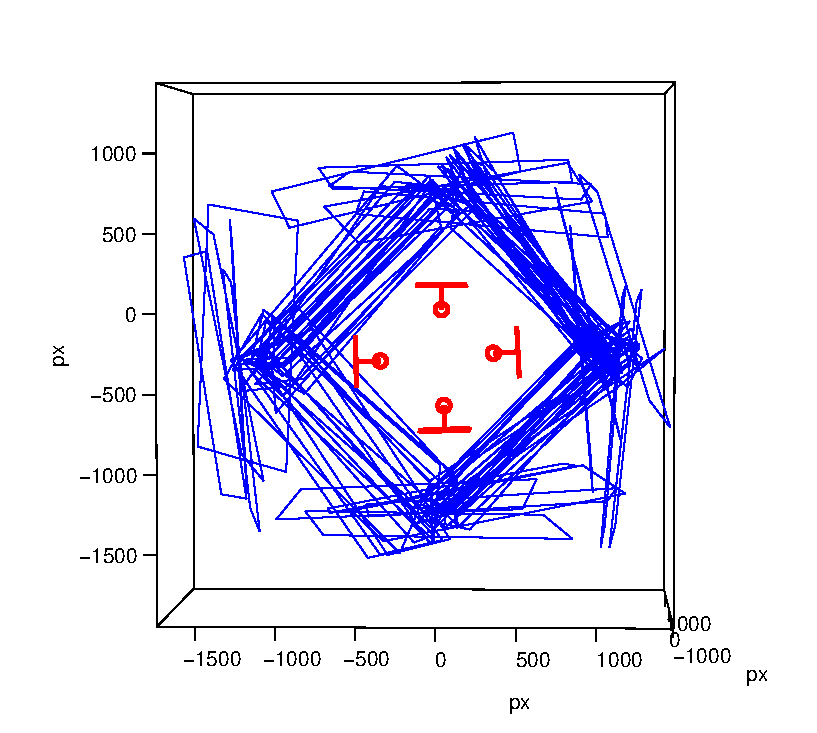
\includegraphics[width=0.47\textwidth]{images/rig1} 
\caption{Two viewpoints of a 3D plot of camera and calibration pattern poses generated by our toolbox for the 4-camera system. } 
\label{fourCameraRigPlot}
\end{figure}



\section{Calibration of a Four-Camera System}
In the second experiment, we validate our toolbox on a four-camera system; neighboring cameras have minimal overlapping fields of view. One camera is a mvBlueFOX camera while the rest are Point Grey Firefly MV cameras. This system is shown in figure \ref{fourCameraRigPhoto}. All the four cameras are normal pinhole cameras. Existing camera calibration toolboxes are difficult to use when it comes to calibrating such systems. 15 image pairs are taken for each pair of neighboring cameras; two examples are shown in figure \ref{fourCameraRigImageFig}. Due to the non-overlapping field of view, neighboring cameras only see a small part of the board close to the board's border. Thus, some images do not have sufficient features for matching, and are automatically discarded by the toolbox. In addition, to ensure accurate intrinsic calibration, we take 5 images for each camera with the pattern occupying a large part of each image. Figure \ref{fourCameraRigPlot} plots the 3D poses of both cameras and patterns. The average reprojection error over all images and corresponding to the estimated intrinsics and extrinsics is $0.7$ pixels. 

\begin{figure}
\centering 
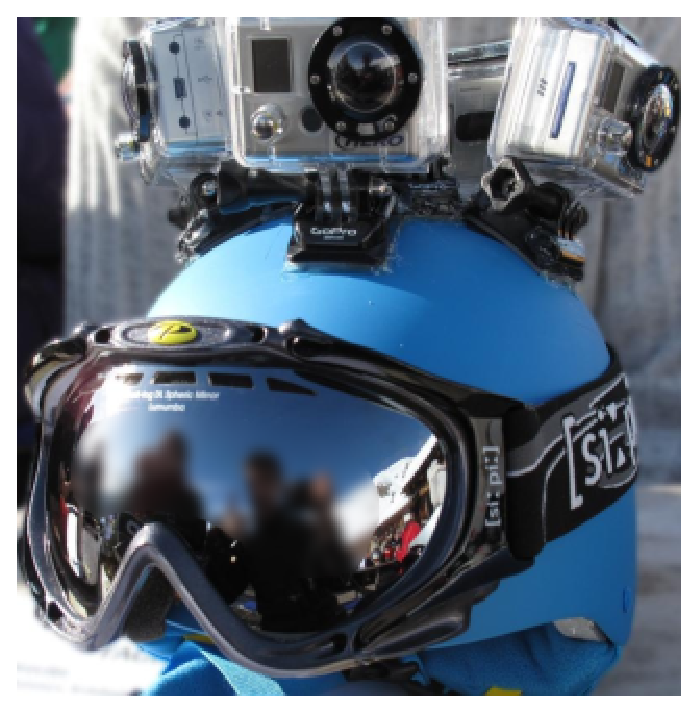
\includegraphics[width=0.57\textwidth]{images/helmet} 
\caption{A 5-camera system mounted on a ski helmet}. 
\label{helmetPhoto}
\end{figure}


\begin{figure*}
\centering
%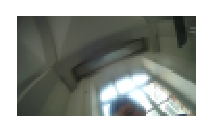
\includegraphics[width=0.115\textwidth]{images/sampleimage/9-1} 
%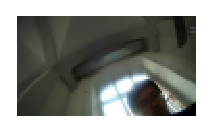
\includegraphics[width=0.115\textwidth]{images/sampleimage/32-1} 
%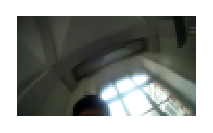
\includegraphics[width=0.115\textwidth]{images/sampleimage/48-1} 
%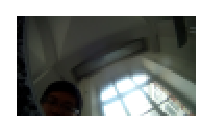
\includegraphics[width=0.115\textwidth]{images/sampleimage/67-1} 
%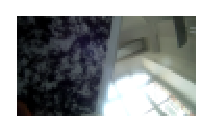
\includegraphics[width=0.115\textwidth]{images/sampleimage/125-1} 
%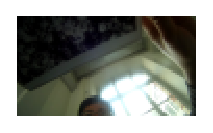
\includegraphics[width=0.115\textwidth]{images/sampleimage/155-1} 
%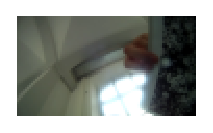
\includegraphics[width=0.115\textwidth]{images/sampleimage/197-1} 
%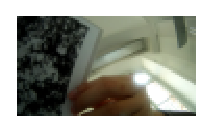
\includegraphics[width=0.115\textwidth]{images/sampleimage/204-1} \\ \vspace{4pt}
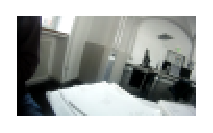
\includegraphics[width=0.115\textwidth]{images/sampleimage/9-2} 
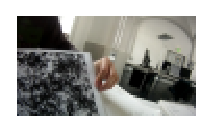
\includegraphics[width=0.115\textwidth]{images/sampleimage/32-2} 
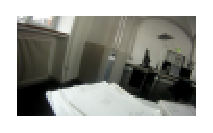
\includegraphics[width=0.115\textwidth]{images/sampleimage/48-2} 
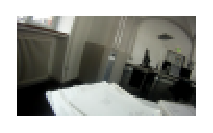
\includegraphics[width=0.115\textwidth]{images/sampleimage/67-2} 
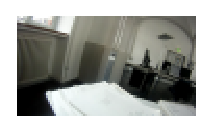
\includegraphics[width=0.115\textwidth]{images/sampleimage/125-2} 

\includegraphics[width=0.115\textwidth]{images/sampleimage/155-2} 

\includegraphics[width=0.115\textwidth]{images/sampleimage/197-2} 
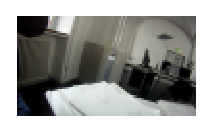
\includegraphics[width=0.115\textwidth]{images/sampleimage/204-2} \\ \vspace{4pt}
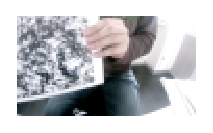
\includegraphics[width=0.115\textwidth]{images/sampleimage/9-3.eps} 
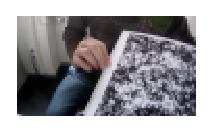
\includegraphics[width=0.115\textwidth]{images/sampleimage/32-3} 
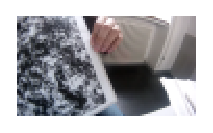
\includegraphics[width=0.115\textwidth]{images/sampleimage/48-3} 
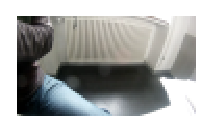
\includegraphics[width=0.115\textwidth]{images/sampleimage/67-3} 
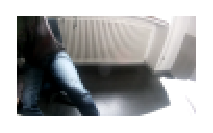
\includegraphics[width=0.115\textwidth]{images/sampleimage/125-3} 
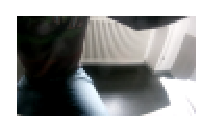
\includegraphics[width=0.115\textwidth]{images/sampleimage/155-3} 
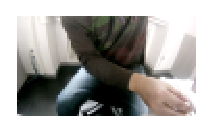
\includegraphics[width=0.115\textwidth]{images/sampleimage/197-3} 
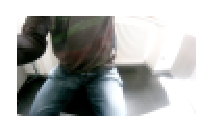
\includegraphics[width=0.115\textwidth]{images/sampleimage/204-3} \\ \vspace{4pt}
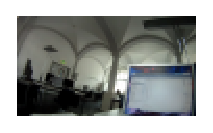
\includegraphics[width=0.115\textwidth]{images/sampleimage/9-4} 
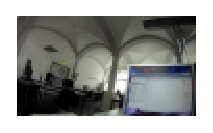
\includegraphics[width=0.115\textwidth]{images/sampleimage/32-4} 
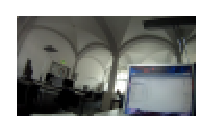
\includegraphics[width=0.115\textwidth]{images/sampleimage/48-4} 
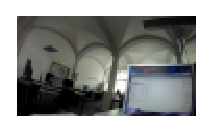
\includegraphics[width=0.115\textwidth]{images/sampleimage/67-4} 
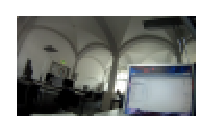
\includegraphics[width=0.115\textwidth]{images/sampleimage/125-4} 
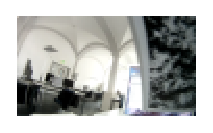
\includegraphics[width=0.115\textwidth]{images/sampleimage/155-4} 
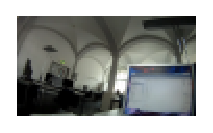
\includegraphics[width=0.115\textwidth]{images/sampleimage/197-4} 
\includegraphics[width=0.115\textwidth]{images/sampleimage/204-4} \\ \vspace{4pt}
\includegraphics[width=0.115\textwidth]{images/sampleimage/9-5} 
\includegraphics[width=0.115\textwidth]{images/sampleimage/32-5} 
\includegraphics[width=0.115\textwidth]{images/sampleimage/48-5} 
\includegraphics[width=0.115\textwidth]{images/sampleimage/67-5} 
\includegraphics[width=0.115\textwidth]{images/sampleimage/125-5} 
\includegraphics[width=0.115\textwidth]{images/sampleimage/155-5} 
\includegraphics[width=0.115\textwidth]{images/sampleimage/197-5} 
\includegraphics[width=0.115\textwidth]{images/sampleimage/204-5} \\ \vspace{4pt}
\includegraphics[width=0.115\textwidth]{images/sampleimage/9-6} 
\includegraphics[width=0.115\textwidth]{images/sampleimage/32-6} 
\includegraphics[width=0.115\textwidth]{images/sampleimage/48-6} 
\includegraphics[width=0.115\textwidth]{images/sampleimage/67-6} 
\includegraphics[width=0.115\textwidth]{images/sampleimage/125-6} 
\includegraphics[width=0.115\textwidth]{images/sampleimage/155-6} 
\includegraphics[width=0.115\textwidth]{images/sampleimage/197-6} 
\includegraphics[width=0.115\textwidth]{images/sampleimage/204-6} 
\caption{Sample images used for calibrating the helmet-mounted five-camera system. Each row corresponds to images from an unique camera. Each column corresponds to images with a common timestamp. }
\label{helmetImageFig}
\end{figure*}

\begin{figure}
\centering 
\includegraphics[trim=0in 0in 0in 0.4in, clip=true, width=0.49\textwidth]{images/5rig1} 
\includegraphics[width=0.47\textwidth]{images/5rig2} 
\caption{Two viewpoints of a 3D plot of camera and calibration pattern poses generated by our toolbox for the 5-camera system. } 
\label{fiveCameraRigPlot}
\end{figure}

\section{Calibration of a Five-Camera System}
The the third experiment, we validate our toolbox on a five-camera system made up of wide angle cameras. The cameras are mounted as a rig on a ski helmet, as is shown in figure \ref{helmetPhoto}. The cameras are five GoPro 2 cameras, under wide angle mode. We take 5 videos from the cameras of a moving calibration pattern. The videos are then synchronized by aligning the audio signal. Figure \ref{helmetImageFig} shows some sample images take from the videos. Each row corresponds to one camera. Each column corresponds to one timestamp after synchronization. The generic camera model is used for single camera calibration. Figure \ref{fiveCameraRigPlot} plots the 3D poses of both cameras and patterns. 


\chapter{Conclusions}
We have proposed a calibration technique using a feature descriptor-based calibration pattern. This technique can be used for calibrating multiple-camera systems. We show our calibration to work successfully with two multiple-camera systems: a normal stereo camera with a large overlapping field of view, and a four-camera system with minimal overlapping fields of view. A toolbox based on our proposed method is available online at {\small{\url{https://sites.google.com/site/prclibo/toolbox}}}. 

%\chapter{Acknowledgement}
%The second author was funded by the DSO National Laboratories Postgraduate Scholarship. In addition, this work was supported in part by the European Community's Seventh Framework Programme (FP7/2007-2013) under grant \#269916 (V-Charge).

\appendix
\chapter{Multiple-Camera System Calibration Toolbox Documentation}

See the next page for the documentation. Its online version is available at {\small{\url{https://sites.google.com/site/prclibo/toolbox/doc}}}

\includepdf[pages=-, frame=true, scale=0.72, pagecommand={\thispagestyle{plain}}, trim=0.6in 0.6in 0.6in 0.6in, clip=true]{doc}

\chapter{Some Explorations on Calibration Using a LCD Display}
The flat screen and good brightness quality of LCD displays is very suitable for displaying calibration pattern. In this part, we show some exploration on using LCD displays for calibration. The main idea of exploiting a LCD display in calibration is to achieve more correspondences in calibration. 

In general, more correspondences result in more accurate and stabler calibration result. Calibration patterns such as chessboard or our features-based pattern usually provide no more than 1000 correspondences. In some recent study, researchers propose some techniques of generating much denser correspondences in calibration.  For example, \cite{grosse2012camera} uses temporal code for indexing points on a display and can achieve very dense correspondences. This techniques is not very convenient as it requires the camera to be fixed on tripod and take video at different poses to percept the entire temporal code. 

Another aspect to achieve dense correspondences is to render the reprojected calibration pattern and compare it with the original pattern. \cite{schiller2008calibration} has done some similar work using chessboard pattern. To render a reprojected calibration pattern, we firstly calibrate the camera using normal correspondences like chessboard corners. Thus the camera intrinsics as the chessboard pose are both known. Then the chessboard photo can be reprojected back to the pattern plane. The reprojected pattern is very similar to the original pattern, with only small deviation or difference due to the initial calibration precision. Thus we have a pixel-wise correspondence between the two images. It is then possible to refine the calibration result by minimizing the summation of pixel-wise difference, such as SSD or SAD, between the reprojected pattern and the original pattern. 

In this chaper, we mainly focus on this above aspect of refining calibration by minimizing the SSD between the original pattern and the reprojected pattern. First we provide a formulation of the refinement problem. For a point $(X, Y)^\top$ on the calibration pattern, its corresponding image point $(u(X, Y), v(X, Y))^\top$ can be obtained via equations \ref{cmEqn1}, \ref{ray2homo1}, \ref{ray2homo2}, \ref{cmEqn2}, and \ref{cmEqn3}. The SSD between reprojected pattern and the original pattern is: 
\begin{equation}
SSD_{I_p}(I_\text{im}) = \sum_{X, Y} \left(I_p(X, Y) - I_\text{im}(u(X, Y), v(X, Y))\right)^2
\end{equation}
where $I_p$ is the original pattern image and $I_\text{im}$ is a photo of the pattern. Thus the refinement stage can be formed as: 
\begin{equation}
\min_{K, D, R_i, t_i, \forall i} \sum_{i} SSD_{I_p}(I_\text{im}^i)
\label{SSDObjEqn}
\end{equation}
where $i$ is the index of each image. $K$ is the camera intrinsics matrix and $D$ is the set of camera distortion parameters. $u$ and $v$ are related by $K$, $D$, $R_i$ and $t_i$. $I_p$ and $P_\text{im}$ are denoted by the grayscale value.

The above equation provides a simple formulation for refining the calibration result by comparing grayscale between all the pixels in the original pattern and the reprojected pattern. Note that in general the grayscale difference between the original pattern and the reprojected pattern is caused by two factors: One is the misalignment of pixels due to the inaccuracy of calibration; The other is the non-linear grayscale conversion from image data to the display output response and from the display output to the photo data. The above equation only considers the first factor of inaccuracy of calibration. We add a grayscale conversion function $f(x, \star)$ to denote the non-linear grayscale conversion for the second factor. Thus the SSD is modified as: 
\begin{equation}
SSD_{I_p}(I_\text{im}) = \sum_{X, Y} \left( f(I_p(X, Y), \star) - I_\text{im}(u(X, Y), v(X, Y)) \right) ^2
\label{newSSDEqn}
\end{equation}
Note that we put a $\star$ in $f$ because the function value is also determined by other factors, which will be discussed next. 

\begin{figure}
\centering
\includegraphics[width=0.9\textwidth, trim=0.5in 7in 1.5in 0in, clip=true]{images/render-flow-chart.pdf}
\caption{A flowchart of the refining the calibration by minimizing the SSD between the original pattern and the reprojected pattern. The left-top pattern is the original pattern. It is shown on a display and captured by camera in to the top-right image. To refine the calibration, the original pattern is converted into the bottom-left pattern, according to the display grayscale response same with the top-right image. The top-right image is reprojected onto the pattern plane as the bottom-right reprojected pattern. Then we minimize the grayscale SSD between the bottom-left converted pattern and the bottom-right reprojected pattern, by refining the calibration result. }
\label{displayFlow}
\end{figure}

Figure \ref{displayFlow} shows a flowchart of how the refinement works. See the figure caption for illustrations. Note that the camera sensor response is not consider since we use the RAW image in our experiment, as will be stated next. 

\section{Explorations on Estimating the Display Output}

\begin{figure}
\centering
\begin{tabular}{ccc}
\includegraphics[width=0.3\textwidth]{images/display-pattern.png}&
\includegraphics[width=0.3\textwidth]{images/display-photo.png}&
\includegraphics[width=0.3\textwidth]{images/rendered.png}\\
(a) & (b) & (c)
\end{tabular}
\begin{tabular}{ccc}
\includegraphics[width=0.3\textwidth]{images/rendered-sample.png}&
\includegraphics[width=0.3\textwidth]{images/fitted-gray.png}&
\includegraphics[width=0.3\textwidth]{images/fitted-image.png}\\
(d)&(e)&(f)
\end{tabular}
\caption{a) An original calibration pattern with noise tiles and solid tiles. b) A raw image photo of the pattern on a display. The RAW image grayscale value is scaled for visualization. c) The reprojected pattern of (b) on the pattern plane. d) Enroded solid tiles of grayscale-255 extracted from (c). e) An visualization of the display grayscale response for grayscale-255 in image (b). This can be interpreted as an interpolation of tile grayscales in (d). f) A pattern generated from the original pattern by converting its grayscale according to the display grayscale response. }
\label{displayPattern}
\end{figure}

The active-matrix liquid-crystal display (AMLCD) is the current mostly used computer display techniques, on either notebooks or desktops. The AMLCD is advantageous for its low weight, good image quality, wide color gamut and good response time. The narrow viewing angle is one of the drawbacks for all LCD techniques. The displays have the best brightness when viewing in its front. When viewing from side, the brightness will be very low. 

We base our study on normal desktop display of AMLCD. In our study, we assume that on the display, all pixels are ideally the same and the background light is uniform. Thus the brightness of each pixel is only determined by the input image grayscale and the viewing angle. 

We show here a experiment of estimating the display response $f$ for different input grayscale values. Three variables are considered: the horizontal viewing angle, the vertical viewing angle and the input grayscale. Thus the $\star$ in the $f$ function in equation \ref{newSSDEqn} represents for the two viewing angle. Consider a coordinate system with its $xy$ plane aligned with the screen. For a pixel $(X, Y, 0)^\top$ and a camera position $(X_c, Y_c, Z_c)^\top$, the horizontal viewing angle is $\text{atan2}(Z_c, X_c - X)$ and the vertical viewing angle is $\text{atan2}(Z_c, Y_c - Y)$. In addition, in the experiment we only consider 4 grayscales of 0, 85, 170 and 255 for simplicity. A special pattern made up with the four grayscales is designed for this experiment, as shown in figure \ref{displayPattern}(a). 

The pattern is composed by noise tiles and solid grayscale tiles. Feature correspondences are detected from the noise tiles. These features are used to generate a initial calibration using our proposed calibration toolbox APIs. The solid grayscale tiles are used for measure the display grayscale response of the four input grayscales on the pattern. Solid grayscale tiles of grayscales 0, 85, 170 and 255 are arranged periodically so that they are uniformly distributed on the pattern. 

The pattern is shown on a LCD display. We execute our experiments on different displays including a Samsung Display 2443BW, a Samsung Display 204B and a Lenovo Ideapad laptop display, with similar results. A DMC-GF2 camera is used for capturing images. To remove the non-linear camera perception, RAW images are used in this experiment so that the display irradiance is linear with the RAW image reading value. Under this setting, our measured $f$ only consists the non-linear grayscale conversion from image data to the display output response. 

6 photos are taken around the display and the camera is firstly calibrated using features detected from noise tiles on the pattern. Figure \ref{displayPattern}(b) shows a sample photo of the displayed pattern. Then the 6 photos are reprojected to the pattern plane using the initial calibration result, as shown in figure \ref{displayPattern}(c). Each solid grayscale tile 	in the reprojected pattern provides a small stable region for measuring the display response for a input grayscale at some viewing angles. For example, figure \ref{displayPattern}(d) shows the eroded region of the tiles in the reprojected pattern corresponding to the grayscale-255 tiles in the original pattern. The solid tiles are eroded because their border maybe misaligned with pixels of other grayscales in the original pattern, due to the inaccruracy of the initial calibration. We collect all the valid pixels from figure \ref{displayPattern}(d). For these pixels, we have the display response grayscale and can also compute their corresponding two viewing angles. Thus we can visualize these pixels in a plot of the response grayscale against the two viewing angles. Figure \ref{displayResponse} shows the plots for the four original pattern grayscale respectively. The vertical axis is the direct RAW image value. 6 colors correspond to 6 images we take. We can see that 6 images are sufficient to cover all most viewing angles for the display. From the plot we can clearly see that the display response is approximately symmetric at the horizontal direction asymmetric at the vertical direction. 
\begin{figure}
\centering
\begin{tabular}{cc}
\includegraphics[width=0.45\textwidth]{images/response-gs0}&
\includegraphics[width=0.45\textwidth]{images/response-gs85} \\
\includegraphics[width=0.45\textwidth]{images/response-gs170}&
\includegraphics[width=0.45\textwidth]{images/response-gs255}

\end{tabular}
\caption{Samples of the display grayscale response function $f(g, \alpha_x, \alpha_y)$ with different $g$. Top-left: $f(0, \alpha_x, \alpha_y)$. Top-right: $f(85, \alpha_x, \alpha_y)$. Bottom-left: $f(170, \alpha_x, \alpha_y)$, Bottom-right: $f(255, \alpha_x, \alpha_y)$. The dots correspond to the small tiles in figure \ref{displayPattern}(d). Different color corresponds to different images. }
\label{displayResponse}
\end{figure}

Denote the horizontal viewing angle as $\alpha_x$ and the vertical viewing angle as $\alpha_y$. Figure \ref{displayResponse} provides samples on functions $f(0, \alpha_x, \alpha_y)$, $f(85, \alpha_x, \alpha_y)$, $f(170, \alpha_x, \alpha_y)$ and $f(255, \alpha_x, \alpha_y)$, with $\alpha_x$ and $\alpha_y$ as two unknowns. We could see that the horizontal and the vertical viewing angles can parametrize the display response very well. By using polynomial regression techniques, $f(g, \alpha_x, \alpha_y)$, with $g = 0, 85, 170, 255$ could be well approximated. In our experiment, we use a degree-5 2D polynomial to approximate the response function for each grayscale and use the fitted model to predict display output grayscale for the reprojected pattern. For each pixel in the reprojected pattern, we can predict its display grayscale response for input grayscales  of 0, 85, 170 and 255, using the fitted polynomial of $f(g, \alpha_x, \alpha_y)$. Figure \ref{displayPattern}(e) shows the display grayscale response in each pixel of the reprojected pattern, for the input grayscale of 255. Note that figure \ref{displayPattern}(e) can be interpreted as a interpolation of the grayscale samples in figure \ref{displayPattern}(d). For each pixel in the original pattern, we compute its viewing angles. Then we predict its display response grayscale using its viewing angles according to the fitted $f(g, \alpha_x, \alpha_y)$. Figure \ref{displayPattern}(f) shows an rendered image converted from the original image, using the viewing angle information corresponding to figure \ref{displayPattern}(c). Pixels in figure \ref{displayPattern}(f) corresponds to $f(I_p(X, Y), \star)$ in equation \ref{newSSDEqn}. We can see that this image is very similar to the reprojected pattern. 


\section{Refine the Calibration}
Substituting the regressed $f$ back to equation \ref{SSDObjEqn}, we can now refine the calibration result using optimization method. Note that the optimization can be very computational expensive as for each iteration we have to compute the SSD over all images. An easy way to accelerate this is to execute the optimization only on a subset of image pixels. 

In our experiment, the proposed refinement can significantly reduce the SSD error between the original pattern and the reprojected pattern. This reduced error implies a better calibration accuracy. For camera calibration task with super high accuracy demand, we suggest to use this proposed method to refinement the calibration. 
\bibliographystyle{plain}
\bibliography{main}



\end{document}
